% !TEX program = platex
% 母音入力 + LoRA fine-tuned LLM による超省入力型日本語入力システム（FSS2026 投稿フォーマット）
% コンパイル: platex main.tex && platex main.tex && dvipdfmx main.dvi
\documentclass[a4paper,10pt,twocolumn]{myjarticle2}
\usepackage[dvipdfmx]{graphicx}
\usepackage{multirow}
\usepackage{amsmath,amssymb}
\usepackage{booktabs}
\usepackage{url}
\usepackage{bm}
\usepackage[dvipdfmx]{color}                        % 追加: 黄色背景ハイライト用(dvipdfmxドライバ明示)
\definecolor{tbd}{rgb}{1,1,1}                       % 修正: 黄色ハイライトを消す(背景色を白に)
\newcommand{\TBD}[1]{#1}            % 修正: 黄色ハイライトを消す(中身のみ表示)
\newcommand{\TBDbox}[1]{\par\noindent{#1}\par}  % 修正: 黄色ハイライトを消す
\newcommand{\HL}[1]{#1}             % 未使用(段落単位は \HLbox を使用)
\newcommand{\HLbox}[1]{\par\noindent{#1}\par}  % 修正: 黄色ハイライトを消す
% 追加: header.tex の数式マクロ(\Cup,\Cap,\Vec)が amssymb と衝突するため、読込前に未定義化する
\let\Cup\relax \let\Cap\relax \let\Vec\relax
%ルビ
\def\ruby#1#2{%
  \leavevmode \setbox0=\hbox{\mathstrut#1}\setbox1=\hbox{\tiny#2}%
  \ifdim\wd0>\wd1 \dimen0=\wd0 \else \dimen0=\wd1 \fi
  \hbox{\kanjiskip=\fill
    \vbox{\hbox to \dimen0{\tiny \hfil#2\hfil}%
       \nointerlineskip
       \hbox to \dimen0{\hfil\mathstrut#1\hfil}}}}
% <<DISPLAYSTYLE mathematical characters>>
%\newcommand{\Frac}[2]{\displaystyle\frac{\raisebox{-1.8pt}{$#1$}}{\raisebox{0.8pt}{$\:#2\:$}}}
\newcommand{\Frac}{\displaystyle\frac}
\newcommand{\Prod}{\displaystyle\prod}
\newcommand{\Sum}{\displaystyle\sum}
\newcommand{\Int}{\displaystyle\int}
\newcommand{\Sqrt}[1]{\sqrt{#1\,}}
\newcommand{\Lim}{\displaystyle\lim}
\newcommand{\Cup}{\displaystyle\bigcup}
\newcommand{\Cap}{\displaystyle\bigcap}
\newcommand{\Min}{\displaystyle\min}
\newcommand{\Max}{\displaystyle\max}
\newcommand{\Vec}[1]{\overrightarrow{#1}}
\newcommand{\Vecb}[1]{\mbox{\boldmath $#1$}}
\newcommand{\NumB}[1]{\noindent\fbox{{\large\bf#1}}\hspace{3pt}}
% <<日本式不等号>>
\makeatletter\def\le{\mathrel{\mathpalette\gl@align<}}
\def\ge{\mathrel{\mathpalette\gl@align>}}
\def\gl@align#1#2{\lower.6ex\vbox{\baselineskip\z@skip\lineskip\z@%
\ialign{$\m@th#1\hfil##\hfil$\crcr#2\crcr=\crcr}}}
\makeatother

\def\labelenumi{(\theenumi)}
\def\theenumi{\roman{enumi}}
 % 修正: プリアンブルでは \include ではなく \input を使う
\pagestyle{empty}
\setlength{\topmargin}{6mm}
\setlength{\oddsidemargin}{-4mm}
\setlength{\evensidemargin}{-4mm}
\setlength{\textwidth}{170mm}
\setlength{\headsep}{0pt}
\setlength{\headheight}{0pt}
\setlength{\textheight}{235mm}
\setlength{\columnsep}{5mm}

\begin{document}
\twocolumn[%
\vspace{-20mm}
\begin{center}
{\LARGE\bf 大規模言語モデルを用いた人にやさしい母音ベース省入力日本語インタフェース}
\vspace{2mm}\par\noindent
{\large A Vowel-Based Low-Effort Japanese Text Input Interface Using Large Language Models}
\vspace{2mm}\par\noindent
{\large
\begin{tabular}{cc}
$\bigcirc$ 田中　峻介$^{1}$， & 久保田　直行$^{1}$\\
$\bigcirc$ Tanaka Shunsuke$^{1}$, & Naoyuki Kubota$^{1}$\\
\multicolumn{2}{c}{$^{1}$東京都立大学}\\
\multicolumn{2}{c}{$^{1}$Tokyo Metropolitan University}\\
\end{tabular}}
\vspace{2mm}\par\noindent
\begin{minipage}{150mm}
{\small{\bf Abstract:}
With the widespread use of mobile devices, Japanese text input interfaces play an important role in everyday information interaction. However, software keyboards require many keys to be displayed on a limited screen area. As a result, the visual and touch-sensitive area of each key becomes small, which can increase the likelihood of input errors during touch operation. This issue may be particularly burdensome for older adults, as age-related changes in motor ability can make it difficult to accurately distinguish and press small keys.
In this study, we propose an ultra-low-input Japanese text entry method that uses only vowel information as input. Using a large language model additionally fine-tuned with LoRA, the proposed method estimates and ranks contextually appropriate candidate words from vowel sequences.
This study aims to clarify the feasibility of a vowel-only input interface and its effectiveness as a human-friendly text input support technology.
\par\noindent}
\end{minipage}
\par\noindent
\end{center}
]

\section{緒言}

文字入力は，情報端末を通じて人と人，人と社会をつなぐ最も基本的な行為の一つである．
しかし加齢に伴う運動・視機能の変化，身体的制約，端末や状況によって，
同じ入力操作が大きな負担となることがある．
誰もが負担少なく自分の意思を伝えられることは，生活の質と尊厳を支えるうえで重要であり，
本研究はこうした人間の負担に着目した使いやすい入力支援を目指す．

従来の日本語入力方式（IME）は十分に実用的かつ高性能である．
本研究の問題意識は，IME の変換精度ではなく，
ユーザに要求される\textbf{入力操作量}にある．
すなわち課題は「変換が正しくない」ことではなく，
「人間の側に求められる操作が多い」ことにある．
かな入力は 50 音相当，QWERTY は 26 キー以上，フリック入力は 12 キーと方向操作・習熟を要求する．
これに伴い，小さなキーを正確に押し分ける負担，フリック方向の記憶・習熟の負担，
多数の候補から目的語を探す認知的負荷，多くのキーが画面を占有する視認性低下が生じ，
小型端末，高齢者，身体制約者などでとりわけ重い負担となりうる．
実際，高齢者ではタッチ操作の「文字数字入力」などで加齢に伴う成功率の低下が報告されており\cite{hatakenaka2024touch}，
認知機能の個人差が Web 操作の難しさに影響することも指摘されている\cite{suzuki2009elderly}．

本研究では，入力情報を日本語の 5 母音（\texttt{a, i, u, e, o}）および撥音
（\texttt{n}）にまで削減する．
たとえば「ありがとう」は \texttt{a i a o u} と入力される．
入力に用いるキーを 6 つにまで絞ることで，
スマートフォンの画面においてキーボードが占める割合を大幅に減らすことができ，
一つひとつのキーを大きく配置できる．
これは，小さなキーを正確に押し分けることが負担となりやすい高齢者にとって特に有効と考えられる．
一方で，このとき子音情報や語彙情報の大部分が失われるため，
入力は本質的に曖昧（ファジィ）となり，母音列は一つの文に一対一で対応せず複数の候補へ多義的に広がる． % 追加: ファジィ入力の位置づけを一文に集約
そこで失われた情報を LLM による CTX 推定で補い，
\textbf{母音列からの日本語候補生成・順位付け}として扱う．
これは，正確な読みを人間が打ち込み候補を探す方式から，曖昧な母音IMEを LLM がリランキングして提示する方式への発想の転換であり，
元の文章の完全復元ではなく候補提示型の入力支援として位置づける．

\section{関連研究}

\subsection{日本語入力と省入力インタフェース}
日本語入力ではかな漢字変換が広く用いられ，読み入力から漢字かな交じり文への変換が研究されてきた．
既存の IME は変換精度の面では十分に成熟しており，残された課題はむしろ人間の側に要求される操作量にある．
モバイル環境ではフリック入力が普及し，小型端末向けの省入力手法も検討されている．
携帯端末向けの曖昧入力（T9 など複数文字を 1 キーに割り当てる方式）や，
予測に基づく加速入力（Dasher 等）は，少ない操作量での入力を目指す点で本研究と方向性を共有する．
視線入力や VR/AR 入力では，ポインティングや滞留選択の負荷が大きく，省入力の要請が強い．
これらの省入力インタフェースに共通するのは，端末や状況によらず人間の側に求められる操作を減らし，
より多くの人が負担少なく入力できるようにするという志向である．

\subsection{LLM と LoRA}
大規模言語モデルは文脈に基づく言語の補完・推定に高い性能を示す．
本研究は，曖昧な母音入力に対し，文脈を考慮した候補を生成する目的で LLM を用いる．
予測に基づく入力という観点では，曖昧入力の弁別や
言語モデル駆動の入力が先行するが，
本研究は子音を落とした母音列という極端な省入力を対象とする点が異なる．
モデルの追加学習には LoRA（Low-Rank Adaptation）を用いる．
LoRA は事前学習済み重みを固定し，低ランク行列のみを学習することで，
少ない学習パラメータで効率的にタスク適応を行う手法である．

\subsection{テキスト入力の評価}
テキスト入力手法は，打鍵効率の指標である KSPC（Keystrokes Per Character）や
誤り率により定量評価される．
主観的作業負荷の評価には NASA-TLX，
ユーザビリティの評価には SUS が広く用いられる．
本研究もこれらの枠組みに沿って評価設計を行う．

\section{提案手法}

\subsection{全体構成}
提案システムは，(1) 入力文または読みを母音列へ変換する母音化部，
(2) 母音列（と任意の文脈）から日本語候補を生成・順位付けする LLM 候補生成部，
からなる（図\ref{fig:overview}）．
ユーザは 5 母音と撥音のみを入力し，システムが上位 $k$ 件の候補文を提示する．

\begin{figure}[t]
  \centering
  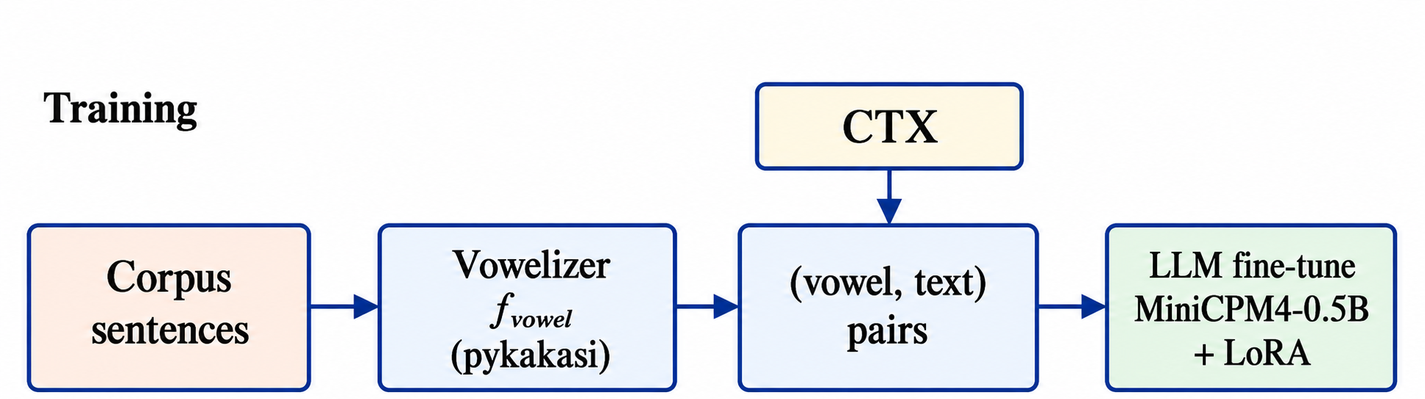
\includegraphics[width=0.95\columnwidth]{figures/fig_overview.png}
  \caption{提案システムの概要．母音列（＋任意の文脈）から上位$k$候補を生成・提示する．}
  \label{fig:overview}
\end{figure}

\subsection{母音化}
入力文または読み列を $x$，母音列を $\bm{v}$ とし，母音化を写像 $f_{\mathrm{vowel}}$ で表す．
\begin{equation}
  \bm{v} = f_{\mathrm{vowel}}(x)
\end{equation}
実装では，漢字を含む任意文を pykakasi により読み（ひらがな）へ変換し，
各かなを 1 母音記号へ写像して空白区切りで出力する．
コードから確認した写像規則は表\ref{tab:vowelrule}の通りである．

\begin{table}[t]
  \centering\small
  \caption{母音化規則}
  \label{tab:vowelrule}
  \begin{tabular}{ll}
    \toprule
    対象 & 扱い \\
    \midrule
    清音・濁音・半濁音 & 母音 \texttt{a/i/u/e/o} に写像 \\
    撥音「ん」 & \texttt{n} \\
    拗音「ゃゅょ」 & 2 文字を 1 母音に集約（例 きょ$\to$\texttt{o}）\\
    促音「っ」 & 無視（出力しない）\\
    長音「ー」 & 無視（例 コーヒー$\to$\texttt{o i}）\\
    小書き「ゎゕゖ」 & 無視 \\
    カタカナ & 一旦ひらがな化して母音化 \\
    句読点・記号 & 出力に現れない \\
    数字・英字 & 読みが付かず脱落（例 100$\to$空，ABC$\to$空）\\
    \bottomrule
  \end{tabular}
\end{table}

この写像により，「今日は天気が悪かった」は
\texttt{o n i i a e n i a a u a a} となる．
子音・濁清の区別が失われるため，同一母音列に複数の日本語表現が対応する
本質的曖昧性が生じる（「寒い」「暑い」$\to$\texttt{a u i}）．

\subsection{候補生成と順位付け}
母音列 $\bm{v}$ から日本語文 $y$ を生成する条件付き分布 $P_\theta(y\mid \bm{v})$ を LLM で表す．
最尤候補は
\begin{equation}
  \hat{y} = \arg\max_{y} P_\theta(y \mid \bm{v})
\end{equation}
であり，上位 $k$ 件の候補集合を
\begin{equation}
  \mathcal{Y}_k(\bm{v}) = \operatorname*{TopK}_{y} P_\theta(y \mid \bm{v})
\end{equation}
と定義する．実装ではビーム探索（ビーム幅 8）により $\mathcal{Y}_k$ を生成し，
重複を除いた上位 $k$ 件を候補として提示する．
任意で直前の文を文脈 $c$ として与えられ，その場合は $P_\theta(y\mid \bm{v}, c)$ を用いる．

\subsection{LoRA による追加学習}
候補生成器は事前学習済み LLM を LoRA で追加学習して得る．
事前学習済み重みを $W$，学習対象の低ランク行列を $A, B$，rank を $r$，スケーリング係数を $\alpha$ とすると，
\begin{equation}
  W' = W + \Delta W = W + BA
\end{equation}
\begin{equation}
  h = Wx + \frac{\alpha}{r}BAx
\end{equation}
であり，$W$ を固定して $A, B$ のみを学習する．
これにより全パラメータ更新に比べ少ない学習量でタスク適応が可能となる．
本研究では母音列$\to$文の生成を教師あり微調整（SFT）として学習し，
損失はプロンプト部をマスクして文（と EOS）部にのみ与える．

\section{評価実験}

提案手法を二つの観点から評価する．
一つは，学習済みモデル単体の性能を評価セット上で測る\textbf{オフライン評価}であり，
候補の正解一致率（Acc@$k$）と入力効率（KSPC）を指標に，
文脈・ビーム幅・LoRA の寄与をアブレーションで切り分ける．
もう一つは，実利用者の操作を要する\textbf{実ユーザ実験}であり，
母音入力に特有の認知負荷を計測 Web アプリを用いて測定する．
本章では評価指標（\ref{subsec:metrics}節）と比較対象（\ref{subsec:compare}節），
実ユーザ実験の設計（\ref{subsec:user}節）を述べ，結果は次章にまとめる．

\subsection{評価指標}
\label{subsec:metrics}
候補提示型の入力支援であることを踏まえ，Top-1 の完全一致だけでなく
Top-3 / Top-5 を重視する．母音入力 $\bm{v}_i$，正解 $y_i$，上位 $k$ 候補集合 $\mathcal{Y}_k(\bm{v}_i)$ に対し，
\begin{equation}
  \mathrm{Acc@}k = \frac{1}{N}\sum_{i=1}^{N}\mathbf{1}\!\left[y_i \in \mathcal{Y}_k(\bm{v}_i)\right]
\end{equation}
を用いる．

入力効率は KSPC（Keystrokes Per Character）で評価する．
\begin{equation}
  \mathrm{KSPC} = \frac{K}{C}
\end{equation}
ここで $K$ は打鍵数，$C$ は正解文字数である．
本稿では誤りなしで入力し切るのに必要な最小打鍵数を $K$ とする理想 KSPC を用い，
提案手法（$K$＝母音キー数）と既存IME方式（ローマ字＝訓令式，JIS かな，フリック，トグル）を
同一の正解文字数 $C$ のもとで比較する．

\subsection{比較対象と実装状況}
\label{subsec:compare}
入力効率（KSPC）については，提案手法（母音入力）に加え，
既存IME方式（ローマ字＝訓令式，JIS かな入力，フリック入力，トグル入力）の
理想 KSPC（誤りなしの最小打鍵数 $\div$ 正解文字数）を
同一評価セット上から自動算出する．
各方式の打鍵数は正解文の読み（pykakasi により取得）から数え，
分母はどの方式も素の正解文字数 $\mathrm{len}(\text{gold})$ で共通とする．
数字・英字を含む文は母音化で情報が脱落し KSPC が不当に小さくなるため評価対象から除外する．
算出結果は次章の表\ref{tab:input}に示す．

\subsection{実ユーザ実験（認知負荷評価）}
\label{subsec:user}
実利用者の操作を要する評価として，参加者 5 名を対象に実験を行った。
本実験用に，スマートフォン／PC のブラウザから実行する
計測 Web アプリを実装した。
各参加者は 4 つの入力方式（ひらがな入力，母音入力，
標準IME，母音入力＋LLM 推論）で課題文（計 9 文）を入力した。

\subsubsection{評価の目的}
本評価の目的は，母音入力に特有の認知負荷を 2 種類に分離して測定することである。
提案手法である母音入力方式では，従来の日本語 IME には存在しない認知的処理が要求される。
具体的には，利用者は入力したい文章を母音列へ変換し，その母音列を保持しながら入力を行う必要がある。
そのため本研究では，入力精度や入力速度だけでなく，利用時の認知負荷についても評価を行う。
認知負荷の評価にあたっては，広く利用されている主観評価手法である
NASA-TLXを参考にした。
ただし本研究では母音入力特有の負荷を分析するため，一般的な精神的負荷を評価するだけでなく，
\textbf{母音変換負荷}（提示文を母音列へ変換する音韻変換の負荷）と
\textbf{記憶保持負荷}（母音列を保持しながら入力するワーキングメモリ負荷）を
独立した評価項目として設計した点に特徴がある。
この分離により，母音入力の負担がどこから生じるのかを切り分けて議論できる。

\subsubsection{リサーチクエスチョン}
\begin{itemize}
  \item \textbf{RQ1}：母音入力は通常 IME と比較して入力効率を向上させるか。
  \item \textbf{RQ2}：母音入力における認知負荷はどこから生じるか（母音変換負荷か記憶保持負荷か）。
  \item \textbf{RQ3}：文章長の増加によって，母音変換負荷と記憶保持負荷はどのように変化するか。
\end{itemize}

\subsubsection{実験設計}
実験は次の 2 種類を実施する。
\paragraph{(1) 従来 IME との比較（RQ1）}
提案手法の有効性を検証するため，通常の日本語 IME 入力と母音入力を比較する。
評価項目は入力時間，正答率，および主観評価とする。

\paragraph{(2) 母音入力内での認知負荷分析（RQ2，RQ3）}
母音入力方式において，文章長による認知負荷の変化を分析する。
課題文を Level~1：単語（例「おはよう」「電話」），
Level~2：10 文字以内の短文（例「今から帰る」「気をつけてね」），
  Level~3：一般文（例「来週はパソコンを買いに行く」）
の 3 段階に分類した。
本設計の要点は，記憶保持負荷を意図的に課すために，
課題文を一定時間提示した後に画面から隠し，記憶した状態で入力させる点にある。
これにより，文を見ながら入力する場合には現れない記憶保持の負荷を顕在化させ，
母音変換負荷と分離して観察できる。

\subsubsection{客観指標と負荷の対応}
計測アプリは試行ごとに次を記録する。これらは 2 種類の認知負荷の代理指標を与える。
\begin{itemize}
  \item 初動時間 $T_{\mathrm{init}}$（課題文を隠した後から最初の打鍵まで）と
        母音化誤り率 $\mathrm{CER}_{\mathrm{vowel}}$
        （被験者が打った母音列と正解母音列\footnote{母音化規則により算出。}の
        編集距離を参照長で正規化した値）は
        \textbf{母音変換負荷}を反映する。
  \item 総入力時間 $T_{\mathrm{total}}$，正答率，候補選択順位は総合的な効率を反映する。
\end{itemize}

\subsubsection{主観評価項目}
各タスク終了後に，以下の項目について 7 段階評価
（1：全くそう思わない～7：非常にそう思う）を実施する。
母音入力条件（7 項目）：(1) 提示された文章を母音列に変換するのは難しかった（母音変換負荷），(2) 母音列を覚えながら入力するのは難しかった（記憶保持負荷），(3) 入力操作そのものは難しかった，(4) 入力中に混乱やストレスを感じた，(5) 入力後に疲れを感じた，(6) 通常の日本語入力より効率的だと感じた，(7) 日常的に利用したいと思った。
通常 IME 条件（3 項目）：(1) 入力操作そのものは難しかった，(2) 入力中に混乱やストレスを感じた，(3) 入力後に疲れを感じた。
このように，母音変換負荷と記憶保持負荷を独立した項目として測ることで，
単一の精神的負荷尺度では区別できない負荷の由来を分離して分析できる。

\subsubsection{解析方針}
参加者数は 5 名と限られるため，統計的検定によって母集団レベルの有意差を
主張することは本研究の射程としない。代わりに，各方式・各 Level の平均値と
参加者ごとの傾向にもとづいて記述的に分析し，
母音入力に固有の負荷構造を観察することを目的とする。
特に，総入力時間 $T_{\mathrm{total}}$・初動時間 $T_{\mathrm{init}}$・打鍵数と，
母音変換負荷・記憶保持負荷の主観評価について，
推論なし条件（ひらがな入力 対 母音入力）と
推論あり条件（標準 IME 対 母音入力＋推論）に分けて比較し，
母音入力のボトルネックが音韻変換と記憶保持のいずれにあるかを議論する。

\section{結果と考察}

% 追加: 主観評価(7段階)を横バーで可視化するマクロ。第1引数=平均値(0-7)。
% 全長 \likertfull を 7 段階に対応させ，値に比例した塗り(濃灰)+残り(淡灰)で表示する。
\newlength{\likertfull}\setlength{\likertfull}{24mm}
\newcommand{\likert}[1]{%
  \begingroup
  \setlength{\fboxsep}{0pt}%
  \colorbox[gray]{0.45}{\rule{0pt}{7pt}\hspace{\dimexpr #1\likertfull/7\relax}}%
  \colorbox[gray]{0.88}{\rule{0pt}{7pt}\hspace{\dimexpr \likertfull - #1\likertfull/7\relax}}%
  \endgroup}

\subsection{入力効率（KSPC）}
入力効率は提案手法（母音入力）の KSPC が $1.12$ であり，
ローマ字入力（訓令式，$1.95$），JIS かな入力・フリック入力（いずれも $1.34$），トグル入力（$3.06$）より少なく，
打鍵数の面で省入力が達成できている（表\ref{tab:input}）．

\begin{table}[t]
  \centering\small
  \caption{入力効率比較（KSPC は理想 KSPC＝誤りなし最小打鍵数 $\div$ 文字数．評価セット 1{,}378 文上で算出）}
  \label{tab:input}
  \setlength{\tabcolsep}{4pt}
  \begin{tabular}{p{3.4cm}cc}
    \toprule
    Method & Keys & KSPC \\
    \midrule
    提案手法（母音入力 + LoRA LLM）& 5 + \texttt{n} & 1.12 \\
    ローマ字入力（訓令式）& 26+ & 1.95 \\
    JIS かな入力 / フリック入力 & 12--50 & 1.34 \\
    トグル入力 & 12 & 3.06 \\
    \bottomrule
  \end{tabular}
\end{table}

\subsection{精度評価とアブレーション}
\label{subsec:acc}
文全体の完全一致精度は，基準条件 a（CTXあり・ビーム 8，提案手法）で
Acc@1 $=7.0\%$，Acc@3 $=11.8\%$，Acc@5 $=14.1\%$ と低く（表\ref{tab:abl}），
母音化による情報欠落の大きさを反映している．これは完全一致ではなく候補提示型支援としての位置づけの妥当性を示す．
LoRA を外した素のベースモデル（条件 e）は Acc@1 が 0\% であり，本タスクが LoRA による追加学習に強く依存することが分かる．
ビーム幅は 4（条件 c）より 8（基準 a），さらに 16（条件 d）の方が高精度であった．
CTX の有無（a と b）では CTX ありが一貫して上回り，CTX の付与が精度向上に寄与することが確認できた（本評価セットは CTX を持つ文を約 32\%＝483 文含む）．

\begin{table}[t]
  \centering\footnotesize
  \caption{精度評価・アブレーション（評価セット 1{,}378 文上の完全一致 Acc@$k$．基準 a が提案手法）}
  \label{tab:abl}
  \setlength{\tabcolsep}{4pt}
  \begin{tabular}{@{}p{4.0cm}ccc@{}}
    \toprule
    Condition & Acc@1 & Acc@3 & Acc@5 \\
    \midrule
    a：CTXあり・ビーム 8（提案手法）& 7.0\% & 11.8\% & 14.1\% \\
    b：CTXなし・ビーム 8 & 5.4\% & 10.0\% & 12.2\% \\
    c：CTXあり・ビーム 4 & 7.0\% & 10.7\% & 11.8\% \\
    d：CTXあり・ビーム 16 & 7.5\% & 13.1\% & 15.2\% \\
    e：LoRA なし（素のベース）& 0.0\% & 0.0\% & 0.0\% \\
    \bottomrule
  \end{tabular}
\end{table}

\subsection{実ユーザ実験結果}
\label{subsec:userresult}
参加者 5 名による各方式・各 Level の試行（正答試行のみ）について，
総入力時間 $T_{\mathrm{total}}$・初動時間 $T_{\mathrm{init}}$・打鍵数の
参加者平均を表\ref{tab:userobj}に，母音入力の主観評価（7 段階）の
参加者平均を表\ref{tab:usersubj}に示す。

\begin{table}[t]
  \centering\small
  \caption{客観指標の参加者平均（$N=5$，正答試行のみ）。母音入力＋推論は打鍵がほぼ 1 で総入力時間が最短。}
  \label{tab:userobj}
  \setlength{\tabcolsep}{4pt}
  \begin{tabular}{p{3.2cm}ccc}
    \toprule
    Method & $T_{\mathrm{total}}$[ms] & $T_{\mathrm{init}}$[ms] & 打鍵数 \\
    \midrule
    ひらがな入力& 6495 & 1224 & 14.1 \\
    母音入力& 6040 & 1539 & 8.2 \\
    標準IME& 6675 & 1100 & 14.9 \\
    母音入力＋LLM推論& 3489 & -- & 1.2 \\
    \bottomrule
  \end{tabular}
\end{table}

\begin{table}[t]
  \centering\footnotesize
  \caption{母音入力の主観評価の参加者平均（$N=5$，7 段階：1=全くそう思わない～7=非常にそう思う）。バーは値に比例（最大 7）。母音変換負荷は高く，候補性能は高く評価された。}
  \label{tab:usersubj}
  \setlength{\tabcolsep}{4pt}
  \begin{tabular}{p{3.8cm}cl}
    \toprule
    項目 & 平均 & \\
    \midrule
    母音変換負荷（変換が難しい）& 4.6 & \likert{4.6} \\
    記憶保持負荷（覚えて入力が難しい）& 3.2 & \likert{3.2} \\
    操作負荷（操作が難しい）& 2.4 & \likert{2.4} \\
    混乱・ストレス & 5.4 & \likert{5.4} \\
    疲労 & 4.6 & \likert{4.6} \\
    \midrule
    候補が出た & 5.4 & \likert{5.4} \\
    候補が上位に出た & 5.2 & \likert{5.2} \\
    候補への信頼 & 4.6 & \likert{4.6} \\
    候補の有用感 & 4.4 & \likert{4.4} \\
    利用意向 & 3.2 & \likert{3.2} \\
    \bottomrule
  \end{tabular}
\end{table}

\subsection{考察}
\subsubsection{推論なしの比較}
まず，推論を介さない 2 方式を比べる。母音入力（推論なし）は
ひらがな入力 に対して打鍵数を $14.1$ から $8.2$ へ確実に削減する一方，
総入力時間は $6495$ ms 対 $6040$ ms とほぼ同等にとどまった。
すなわち母音化によって削減された物理的な打鍵コストは，
文を母音列へ変換し保持する認知コストへと置き換わっており，
省打鍵がそのまま時間短縮には結びつかない。
実際，母音入力（推論なし）は初動時間が長く（$1539$ ms 対 $1224$ ms），
入力前の音韻変換に時間を要していることがうかがえる。

\subsubsection{推論ありの比較}
次に，推論ありの 2 方式を比べる。母音入力＋推論は標準 IME の
$6675$ ms に対し $3489$ ms と約半分の総入力時間で入力を完了し，
打鍵数も平均 $1.2$ とほぼ「母音列を一度打って候補を選ぶ」操作に集約された。
特に IME での入力に時間を要する参加者ほど短縮効果が大きく，
LLM 推論が母音入力の変換・確定コストを肩代わりすることで，所要時間が半減したことから
提案手法が IME として実用的な入力速度に達することが示された。

\subsubsection{ボトルネックの所在}
ただし，母音入力＋推論の初動時間は本実験の計測方式では正しく取得できない。
他方式は打鍵がそのまま確定文字となるため初動時間を音韻変換時間として分離できるが，
母音入力＋推論では打鍵・候補生成・選択・確定が連続し，最初の打鍵までの値が候補を待つ時間を含むため同じ意味で比較できない。
このため初動時間は値を示さず（表\ref{tab:userobj} の ``--''），以降の議論には用いない。
代わりに，母音入力に伴う負荷は推論なしの母音入力から論じる。
この傾向は主観評価とも整合し，母音変換負荷（$4.6$）は高く評価された。
客観・主観の双方から，母音入力のボトルネックは
音韻変換（母音変換）にあることが分かった。
一方で操作負荷は低く（$2.4$），候補が出る・上位に出る・信頼できるといった
候補性能は高く評価された（$5.4$／$5.2$／$4.6$）。
これは提案手法の中核である LLM 候補提示が肯定的に受容されたことを意味する。
他方で混乱・ストレス（$5.4$）や疲労（$4.6$）は高く，
利用意向は中程度（$3.2$）にとどまった。
以上から，提案手法は IME として実用的な速度を達成しつつも，
残る課題は入力操作ではなく母音変換の負担軽減にあると結論づけられる。
なお参加者間の個人差は大きく，本結果は予備的な知見である。

\section{結論}

本稿では，日本語の母音列のみを入力情報とし，
LoRA により追加学習した小型 LLM を用いて
文脈に応じた日本語候補を生成・順位付けする超省入力型日本語入力システムを提案した．
従来 IME の変換精度ではなく入力操作量に着目し，
入力を 5 母音と撥音にまで削減したうえで，
失われた情報を LLM の文脈推定で補う枠組みを示した．
実装としては，CC-100 と字幕コーパスから母音列$\to$文の SFT データを構築し，
MiniCPM4-0.5B を LoRA で追加学習し，ビーム探索により上位 $k$ 候補を提示する系を構築した．
評価については，候補生成精度（Acc@$k$, MRR, CER/WER），
入力効率（KSPC, 入力削減率），UI 効率（キー数，画面占有率），
および認知負荷（NASA-TLX を参考にしつつ，母音変換負荷と記憶保持負荷を
独立に測る主観項目）を従来 IME と比較する枠組みを整備した．

今後の課題は，(1) 評価コードによる定量指標の確定，
(2) Base LLM・頻度 baseline・random baseline との比較実装，
(3) 若年・高齢，フリック熟練・非熟練を含む実ユーザ実験の実施，
(4) 固有名詞・数字・英字に対する補完経路の設計である．


% 参考文献。FSS2026サンプルに合わせ thebibliography 環境で直接記述する。
% note=[要確認] の書誌は原論文PDFで最終確認すること（refs.bib 参照）。
% 並び順: 本文中で \cite が登場する順（01_intro → 02_related_work → 03_method）。
\begin{thebibliography}{99}

% 01_intro: 認知機能評価支援システム
\bibitem{kubota2018cognitive}
\colorbox{tbd}{久保田, 大保, 松田, 万治, 青村, 武田}:  % 修正: 名字のみに統一(黄色ハイライト)
自動車運転再開にむけた認知機能評価支援システム, 2018.

% 01_intro: 高齢者のためのスマートデバイス連動型シニアカー
\bibitem{nakamura2015seniorcar}
\colorbox{tbd}{中村, 田松, 久保田, 坂下}:  % 修正: 名字のみに統一(黄色ハイライト)
高齢者のためのスマートデバイス連動型シニアカー,
ロボティクス・メカトロニクス講演会 (ROBOMECH2015), 2A1-005, 2015.

% 01_intro: タッチ端末操作の操作特性の加齢変化
\bibitem{hatakenaka2024touch}
\colorbox{tbd}{畠中, 高橋, 下村, 原田}:  % 修正: 名字のみに統一(黄色ハイライト)
タッチ端末操作における操作特性の加齢変化 ―2024年度計測結果の報告―,
人間工学, Vol. 61, Suppl., 2024.

% 01_intro: 高齢者の認知特性とWebインタフェース
\bibitem{suzuki2009elderly}
\colorbox{tbd}{鈴木, 本宮, 原, 須藤, 佐藤, 熊田, 北島}:  % 修正: 名字のみに統一(黄色ハイライト)
高齢者の認知特性に適合した Web インタフェースのデザインに関する研究(2) ― 高齢者の認知機能が Web 操作に及ぼす影響 ―,
ヒューマンインタフェースシンポジウム 2009, 2009.

% 02_related_work: 高齢者にも優しい視線入力システム
\bibitem{murata2009gaze}
\colorbox{tbd}{村田, 早見, 森}:  % 修正: 名字のみに統一(黄色ハイライト)
視線入力システムの高性能化・実用化に関する研究 ― 高齢者にも優しい視線入力システムの開発 ―,
岡山大学大学院自然科学研究科, 2009.

% 02_related_work: VR環境での触感を伴ったフリック入力
\bibitem{kiyohara2022vrflick}
\colorbox{tbd}{清原, 沢田, 野呂}:  % 修正: 名字のみに統一(黄色ハイライト)
VR 環境における文字入力のための触感を伴ったフリック入力方法,
日本ソフトウェア科学会第39回大会 (2022年度) 講演論文集, 2022.

% 02_related_work: BubbleGlide（スマートウォッチ向け日本語曖昧入力） % 追加
\bibitem{toba2020bubbleglide}
\colorbox{tbd}{戸羽, 加藤, 山本}:  % 修正: 名字のみに統一(黄色ハイライト)
BubbleGlide: N-gram を用いたスマートウォッチ向け日本語曖昧入力ジェスチャーキーボード,
情報処理学会 インタラクション 2020 (IPSJ Interaction 2020), 2020.

% 02_related_work: 母音・子音の順に選択する間接タッチ用かな入力（WISS 2024） % 追加
\bibitem{wada2024vowelconsonant}
\colorbox{tbd}{和田, 白根, 崔, 志築}:  % 修正: 名字のみに統一(黄色ハイライト)
母音, 子音の順に選択を行う間接タッチ用かな文字入力手法,
インタラクティブシステムとソフトウェアに関するワークショップ (WISS 2024), 2024.

% 02_related_work: InvisiVowel
\bibitem{sugawara2023invisivowel}
\colorbox{tbd}{菅原, 鳴海}:  % 修正: 名字のみに統一(黄色ハイライト)
InvisiVowel: スマートフォンにおけるフリックの母音情報のみを利用したキーボード表示のない入力システム,
第31回インタラクティブシステムとソフトウェアに関するワークショップ (WISS 2023), 2023.

% 02_related_work: 母音列制約付き子音復元（VCCR）
\bibitem{hashimoto2026vccr}
\colorbox{tbd}{橋本}:  % 修正: 名字のみに統一(黄色ハイライト)
機械読唇の精度向上に向けた自然言語処理による母音列からの日本語文復元,
早稲田大学大学院基幹理工学研究科 修士論文, 2026.

% 02_related_work: KSPC（打鍵負担の指標） % 追加
\bibitem{mackenzie2002kspc}
\colorbox{tbd}{I. S. MacKenzie}:  % 追加: イニシャル+名字形式(黄色ハイライト)
KSPC (Keystrokes per Character) as a Characteristic of Text Entry Techniques,
Proceedings of the Fourth International Symposium on Human Computer Interaction with Mobile Devices (LNCS 2411), pp. 195--210, 2002.  % 追加

% 03_method: 学習データ CC-100 (XLM-R) % 追加
\bibitem{conneau2020xlmr}
\colorbox{tbd}{A. Conneau, K. Khandelwal, N. Goyal, V. Chaudhary, G. Wenzek, F. Guzmán, E. Grave, M. Ott, L. Zettlemoyer, V. Stoyanov}:  % 追加: イニシャル+名字形式
Unsupervised Cross-lingual Representation Learning at Scale,
Proceedings of the 58th Annual Meeting of the Association for Computational Linguistics (ACL), pp. 8440--8451, 2020.

% 03_method: 学習データ OpenSubtitles % 追加
\bibitem{lison2016opensubtitles}
\colorbox{tbd}{P. Lison, J. Tiedemann}:  % 追加: イニシャル+名字形式
OpenSubtitles2016: Extracting Large Parallel Corpora from Movie and TV Subtitles,
Proceedings of the Tenth International Conference on Language Resources and Evaluation (LREC 2016), pp. 923--929, 2016.

% 03_method: 学習データ JESC % 追加
\bibitem{pryzant2018jesc}
\colorbox{tbd}{R. Pryzant, Y. Chung, D. Jurafsky, D. Britz}:  % 追加: イニシャル+名字形式
JESC: Japanese-English Subtitle Corpus,
Proceedings of the Eleventh International Conference on Language Resources and Evaluation (LREC 2018), 2018.

% 03_method: LoRA
\bibitem{hu2022lora}
\colorbox{tbd}{E. Hu,} \colorbox{tbd}{Y. Shen,} \colorbox{tbd}{P. Wallis,} \colorbox{tbd}{Z. Allen-Zhu,} \colorbox{tbd}{Y. Li,} \colorbox{tbd}{S. Wang,} \colorbox{tbd}{L. Wang,} \colorbox{tbd}{W. Chen}:  % 修正: イニシャル+名字形式に統一(黄色ハイライト、各著者ごとに囲み行末で折り返す)
LoRA: Low-Rank Adaptation of Large Language Models,
International Conference on Learning Representations (ICLR), 2022.

\end{thebibliography}


%%%%% 連絡先 %%%%%
\vspace{-1mm}\par\noindent
\subsection*{連絡先}
\noindent
\begin{tabular}{l}
田中　峻介（東京都立大学）\\
E-mail: {\tt syunsukeyuto@gmail.com}
\end{tabular}

\end{document}
